\documentclass[a4paper,11pt,aps,tightenlines,nofootinbib]{revtex4}
\usepackage{xspace}
\usepackage[english]{babel}
\usepackage{amsfonts}
\usepackage{amsmath, amsthm, amssymb, mathrsfs}
\usepackage[dvips]{graphicx}
\usepackage{pdfpages}
\usepackage{setspace}
\usepackage{indentfirst}
\usepackage[margin=2.5cm]{geometry}
\usepackage{bbm}

\usepackage{pstricks}
\usepackage{enumerate}
\usepackage{pstricks-add}
\usepackage{epsfig}
\usepackage{caption}
\usepackage{subcaption}
\usepackage{pst-grad}
\usepackage{pst-plot}
\usepackage{physics}

\newcommand{\pun}[1]{\textcolor{red}{\bf #1}}

\begin{document}


%\title{Quantum simulations of topologically non-homeomorphic spacetime atoms in loop quantum gravity}
\title{Quantum simulation of a space-time atom in loop quantum gravity}
\author{Caleb Rotello}
\author{Hakan Ayaz}

\begin{abstract}
\end{abstract}


\maketitle


\section{Introduction}
        A major open problem in NISQ is whether modern quantum computers can practically solve classically intractable problems \cite{nisq}.
        We had access Google's Weber QPU, a 53 qubit superconducting quantum computer. It is the same computer used in \cite{supremacy}. 
        The following is a report of using the Weber QPU to simulate spin-foam amplitudes in Loop Quantum Gravity (LQG). It also serves to 
        analyze whether NISQ computers are fit to simulate LQG.

        Quantum gravity is a field of theoretical physics attempting to find a quantum mechanical description of gravity.
        LQG is a theory based on the quantization of space-time, where entangled quantum tetrahedra give rise to 3+1 dimensional space-time in a way that 
        unifies quantum mechanics and general relativity \cite{ashketar}. Because of the complexity of the Plank scale's degrees of freedom, plus the exponential
        growth in the dimension of a Hilbert space, quantum gravitational systems are too difficult for classical supercomputers \cite{ibm-qsim-qubit-of-space}. 
        However, quantum computation gives an exponential speedup to problems and a dramatic increase in spatial efficiency; two space-time atoms have a wavefunction of 
        $2^{40}$ states. This requires $\sim 8$TB on a classical computer, but only 40 qubits on a quantum computer.


\section{Loop Quantum Gravity}
        We analyze covariant LQG using the spin-foam model. In the spin-foam model,
        3-dimensional space is described by a 3-dimensional quantum space state. Evolution from 
        initial 3-dimensional space states to final 3-dimensional space states creates the 4-dimensional quantum spacetime regions \cite{covariant-lqg}. 
        Spin-foam amplitudes are the probability amplitudes of the spin-foam model after one such evolution.

        Calculation of the spin-foam amplitudes is an essential step to understand the spin-foam model in LQG. Unfortunately, spin-foam amplitudes are 
        exponentially difficult to calculate, making non-trivial spin-foam models impossible for classical computers. That is why quantum computers are 
        the most convenient way to calculate these amplitudes especially superconducting circuits provide a competitive result while building practical quantum computers.

\subsection{Constraints}
        There are 3 constraints in LQG. First is the Gauss constraint, which is used for constraining the spin-networks with the 
        equation $0=P_G \ket{T}$, where $\ket{T}$ is the tensor product state of the spin-network.
        The second constraint is spatial diffeomorphism, which is used for characterizing the topology between all spin networks. 
        The third one is the Hamiltonian constrain which 
        is the most difficult to satisfied, is used for the encodes temporal dynamics of the LQG \cite{diffeo}. 


\subsection{Quantum Tetrahedra and Spin-Networks}
        In any $n$-dimensional space, an $n$-simplex is the shape with the fewest possible number of faces; a 
        2-simplex is a triangle, a 3-simplex is a tetrahedron, and so on to higher dimensions. One central tenet 
        of LQG is quantized space-time, and the tetrahedron is the simplest 3 dimensional geometry that can be used for this quantization. 
        Therefore, to get discrete 3-dimensional space 
        we will choose the 3-simplex, or tetrahedron, to be our discrete unit of space \cite{simplical-decomp}. One tetrahedron is defined by the 
        equation: 
        \begin{equation} 
                \vec J_1 + \vec J_2 + \vec J_3 + \vec J_4 = 0
        \end{equation}
        where $\vec J_i = (J_x,J_y,J_z)$ is the angular momentum vector of the $i$th face \cite{covariant-lqg}. We can then define 
        a quantum tetrahedron, or qubit of space, with the following \cite{qspacetime-on-qsim}, where $\theta$ and $\phi$ are 
        angles on the Bloch sphere: 
        \begin{align}
                &\ket{t} = \cos(\frac{\theta}{2})\ket{0_L} + e^{i\phi}\sin(\frac{\theta}{2}) \ket{1_L}\\
                &\ket{0_L} = \frac{1}{2}(\ket{01}-\ket{10})(\ket{01}-\ket{10})\\
                &\ket{1_L} = \frac{1}{\sqrt{3}}[\ket{1100}+\ket{0011}-\frac{1}{2}(\ket{01}+\ket{10})(\ket{01}+\ket{10})]
        \end{align}
        This quantum tetrahedron is the discrete unit of 3 dimensional quantum space.
        A collection of connected quantum tetrahedra gives rise to a spin-network graph, where each node in the graph is a tetrahedron and links are formed by gluing adjacent faces \cite{gluing-polyhedra}. 
        A spin-network graph is given by the tensor product: 
        \begin{equation}
                \ket{T} = \otimes_{i=1}^N\ket{t_i}
        \end{equation}
        where $N$ is the number of tetrahedra.

        The 4-simplex is a geometric object used to create discrete 3+1 dimensional space-time \cite{simplical-decomp}, so in order to 
        properly simulate LQG spin-foam amplitudes we need to create a 4-simplex with our quantum tetrahedra.
        An $n$-simplex is created by gluing $n+1$ simplices from the $n-1$ dimension; a 2 dimension triangle is created by ``gluing'' 3 lines 
        together. To create the 4-simplex, we will glue 5 quantum tetrahedra together with entanglement between faces. 
        A space-time atom is then the process where $m$ quantum tetrahedra glue to form $5-m$ quantum tetrahedra \cite{covariant-lqg}. Two faces glued together 
        is equivalent to a ``link'' in the spin-network, given by a collection of Bell states:
        \begin{equation}
                \ket{W} = \otimes_{l=1}^{2N} \ket{\epsilon_l}, \; \ket{\epsilon_l} = \frac{\ket{01}-\ket{10}}{\sqrt{2}}
        \end{equation}
        where $\ket{\epsilon_l}$ is a link $l$ in the graph. A 4-simplex forms a maximally entangled spin-network graph of five quantum tetrahedra. 

\subsection{Transition Amplitudes}
        Evolution of 3-dimensional space states corresponding to 3-dimensional boundaries of space-time encode the spin-foam amplitudes, or transition amplitudes, between the 
        initial and final spin-networks. The transition amplitude represents local dynamics of a spin-network \cite{ooguri} by showing the change in probability amplitudes. To satisfy 
        the Gaussian constraint, a spin-foam amplitude is given by:
        \begin{equation}
                A = \bra{\psi}P_G\ket{\psi}
        \end{equation}


\section{Quantum Simulation}
        We performed quantum simulations of spin-networks of two and five quantum tetrahedra to get the spin-foam amplitude of topologically inequivalent spin-networks.
        In order to minimize the errors due to noise and coherence times, we only consider the $\theta=0$ case where $\ket{t} = \ket{0_L}$. One qubit of space is created with 
        the operator $U$ such that $\ket{t} = U\ket{0000}$, and the Bell state is created with operator $B$ such that $\ket{\epsilon} = B\ket{00}$.

        The spin-foam amplitude of a spin-network of quantum tetrahedra is given by the inner-product: %$A=\bra{W}\ket{T}$, or more explicitly
        \begin{equation}
                A = \bra{W}\ket{T}
        \end{equation}
        To simulate this, we first prepare the system in the all zero state, $\ket{0\dots 0}$. We then create $N$ qubits of space by acting with $U$ on sets of 4 qubits.
        A spin-network is then created by maximally entangling the qubits of space with inverse Bells states $B^\dagger$. Finally, we find our amplitude by measuring the 
        final amplitude of the $\ket{0\dots0} $ state. This algorithm is equivalent to the inner-product:
        \begin{equation}
                A = \bra{0\dots0}B^\dagger U\ket{0\dots0}
        \end{equation}
        While the amplitude is given by the inner product, the results from the quantum simulation will be the probability obtained from the amplitude. $\bra{W}\ket{T}$ is the spin-foam 
        amplitude, while $\abs{\bra{W}\ket{T}}^2$ is the probability. 


\subsection{Circuit}
        Our circuit must satisfy as many of the constraints in LQG as possible. The Hamiltonian constraint is currently an active area of research,
        and has been simulated using adiabatic quantum computing \cite{adiabatic}, but it is not considered here. The diffeomorphism constraint is satisfied implicitly in 
        the structure of the circuit \cite{ibm-qsim-qubit-of-space}, and we satisfy the Gauss constraint with the operators $P_G = B^\dagger U$.

        The operators mentioned above are equivalent to the following quantum circuits:
        \begin{figure}[h!]
                \begin{subfigure}[b]{.3\textwidth}
                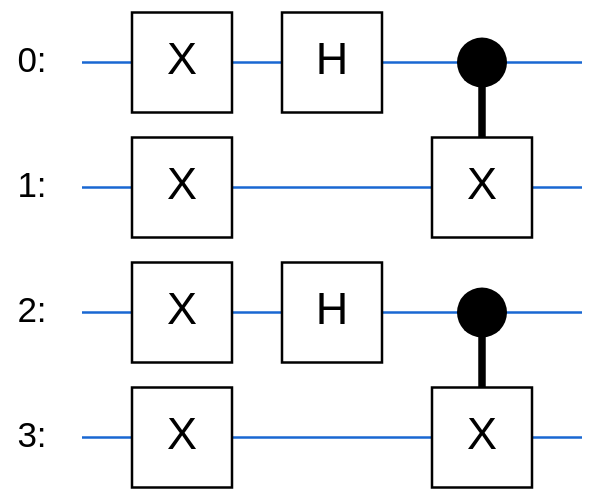
\includegraphics[scale=.3]{images/qtet_state_prep.png}
                \caption{$U_{0-3}$}
                \end{subfigure}
                \begin{subfigure}[b]{.3\textwidth}
                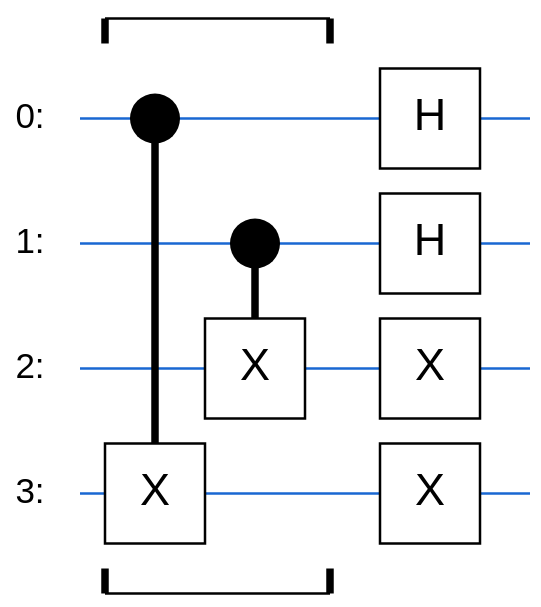
\includegraphics[scale=.3]{images/inv_bell_state.png}
                \caption{$B^\dagger_{03,12}$}
                \end{subfigure}
                \caption{Circuit diagrams \cite{cirq}}
        \end{figure}

        Notice how in the $\ket{0_L}$ state, the entanglement is only within the pairs $(0,1)$ and $(2,3)$. This is part of what makes the $\ket{0_L}$ state trivial;
        the quantum tetrahedron's faces are each only entangled with one other faces. This is not the case for any $\theta\neq 0$ in the $\ket{t}$ state.

\subsection{Topology}
        Spin-networks have different transition amplitudes based on the configuration of links in the graph. In the $\ket{0_L}$ state, when all amplitudes of the wavefunction 
        are uniform, this transition amplitude is a dependent variable of, mostly, the topology of the quantum circuit. In this case, the final wavefunction  
        has uniform amplitudes, so the amplitude of the $\ket{0\dots0}$ state is just a measure of the possible states of the system, like if a card just had $\frac{1}{52}$ on it if it was 
        picked from a full deck, or $\frac{1}{13}$ if it was just picked from a suite of cards. The topology of each of our circuits can be defined by the number of independent ``chains'' 
        of qubits that emerge and form shapes. In our observation, amplitudes of different spin-networks from the same topology can be different up to a sign change. Formal proofs of this 
        will be presented in future work.

\subsection{Dipole Spin Network}
        This can be thought of as the gluing of two quantum tetrahedra, with each face paired to another face. It is the minimal triangulation of the 3-sphere, also known as the 
        dipole cosmology \cite{homogeneity-lqc}. We can organize expected values into two topological groups: one chain and two chains. Expected values are shown in the table below.
        \begin{table}[h]
        \begin{centering}
                \begin{tabular}{|l|l|}
                        \hline
                        Group & $ \abs{\bra{W}\ket{00_L}}^2$\\ \hline
                        Single & 0.0625 \\ \hline
                        Double & 0.015625 \\ \hline
                \end{tabular}
                \caption{Spin-foam amplitude of dipole topological groups}
        \end{centering}
        \end{table}

        The different circuits are shown in figure 2, 
        brown is the connection in state preparation, blue is the connection in the Bell state.

        \begin{figure}[h] \label{dipole-topology}
                \begin{subfigure}[b]{.4\textwidth}
                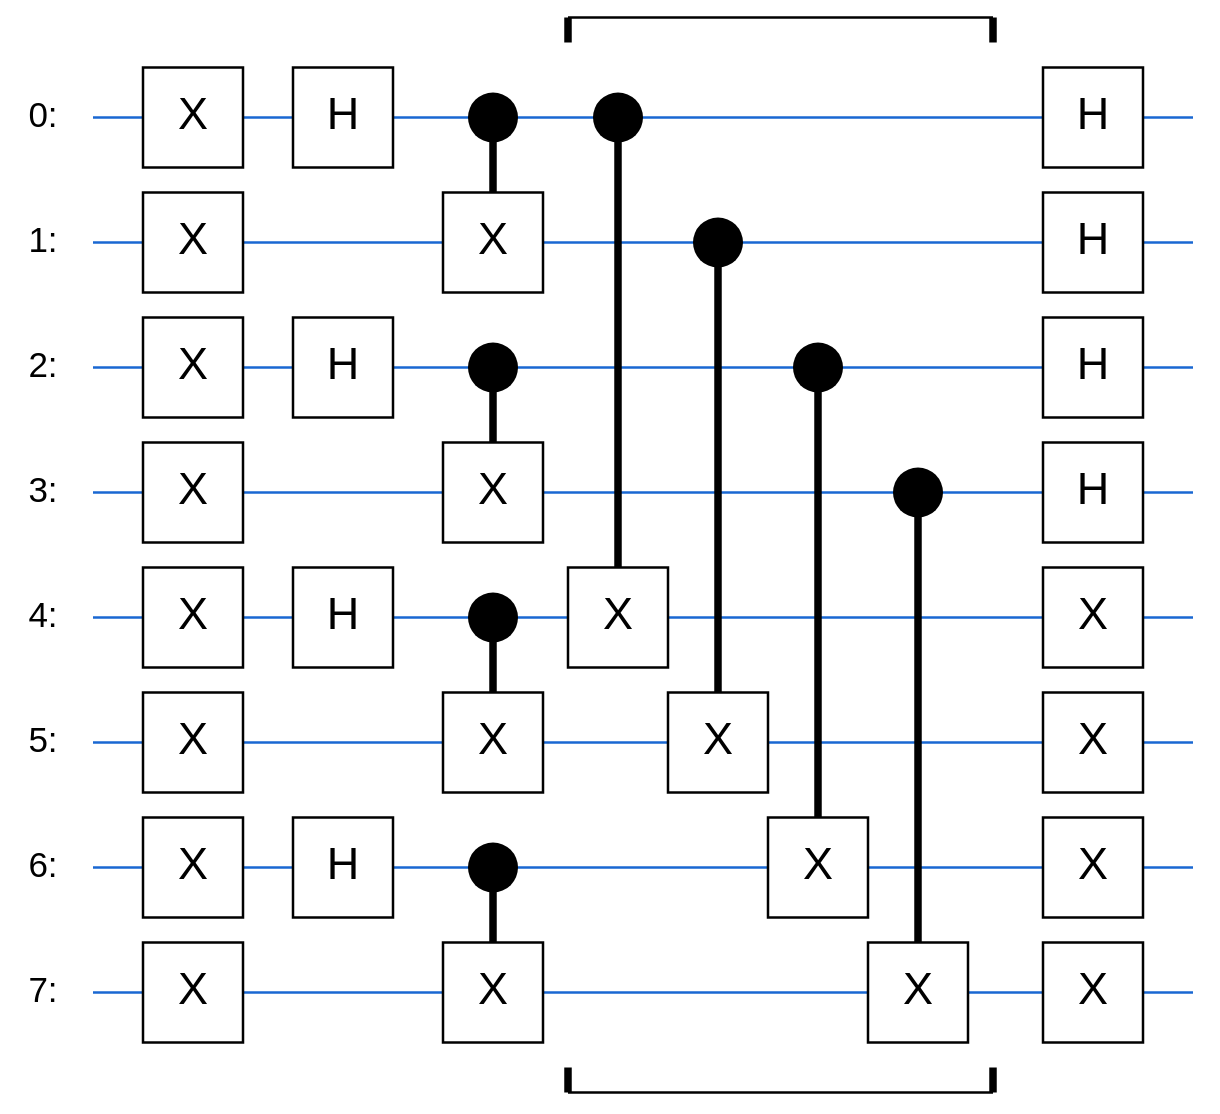
\includegraphics[scale=.2]{images/dipole_disjoint_circuit.png}
                \caption{$B^\dagger_{04,15,26,37}U$ \cite{cirq}}
                \end{subfigure}
                \begin{subfigure}[b]{.3\textwidth}
                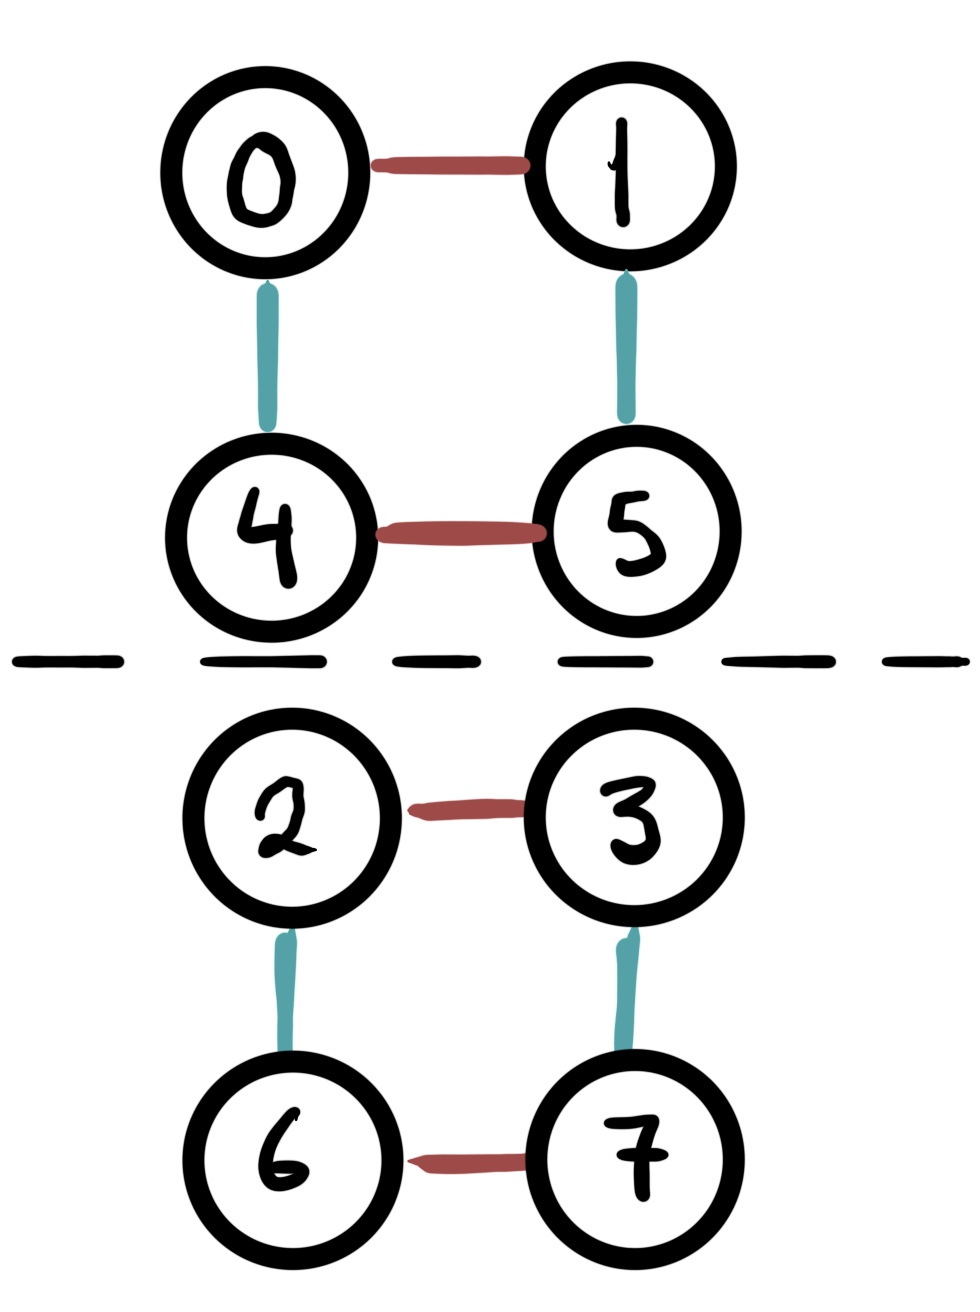
\includegraphics[scale=.1]{images/dipole_disjoint.jpg}
                \caption{Double topology, $04,15,26,37$}
                \end{subfigure}
                \begin{subfigure}[b]{.2\textwidth}
                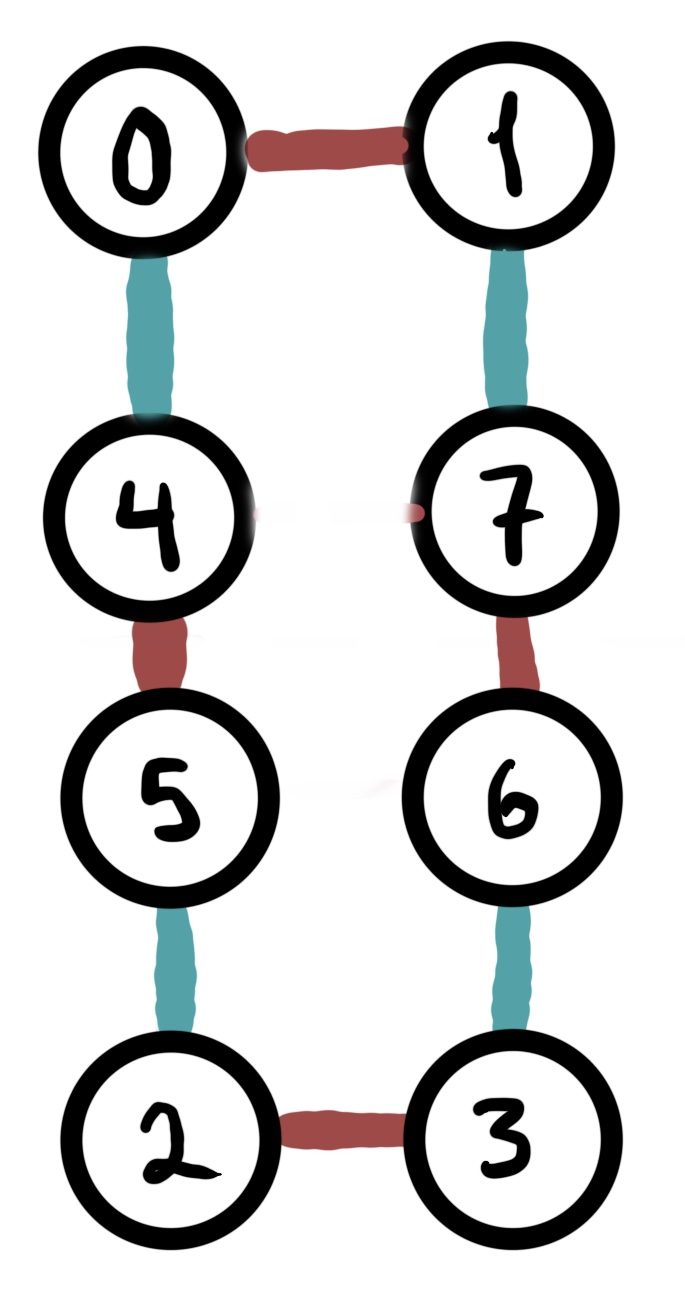
\includegraphics[scale=.1]{images/dipole_union.jpg}
                \caption{Single topology, $04,17,25,36$}
                \end{subfigure}
                \caption{Dipole circuit and topology}
        \end{figure}        


\subsection{4-Simplex Spin Network}
        To simulate a 4-simplex, we simulate the creation of a spin-network 
        with maximum entanglement between the vertices. This is the gluing of five quantum tetrahedra to form a space-time atom. It has topology of one, two, and three chains. Expected values are shown in the table below.

        \begin{table}[h]
        \begin{centering}
                \begin{tabular}{|l|l|}
                        \hline
                        Group & $\bra{W}\ket{00000_L}$\\ \hline
                        Single & $\pm2^{-9}$ \\ \hline
                        Double & $\pm2^{-8}$ \\ \hline
                        Triple & $\pm2^{-7}$ \\ \hline
                \end{tabular}
                \caption{Spin-foam amplitude of 4-simplex topological groups}
        \end{centering}
        \end{table}

        The topological groups correspond to the following circuits


        \begin{figure}[h] \label{simplex-topology}
                \begin{subfigure}[b]{.3\textwidth}
                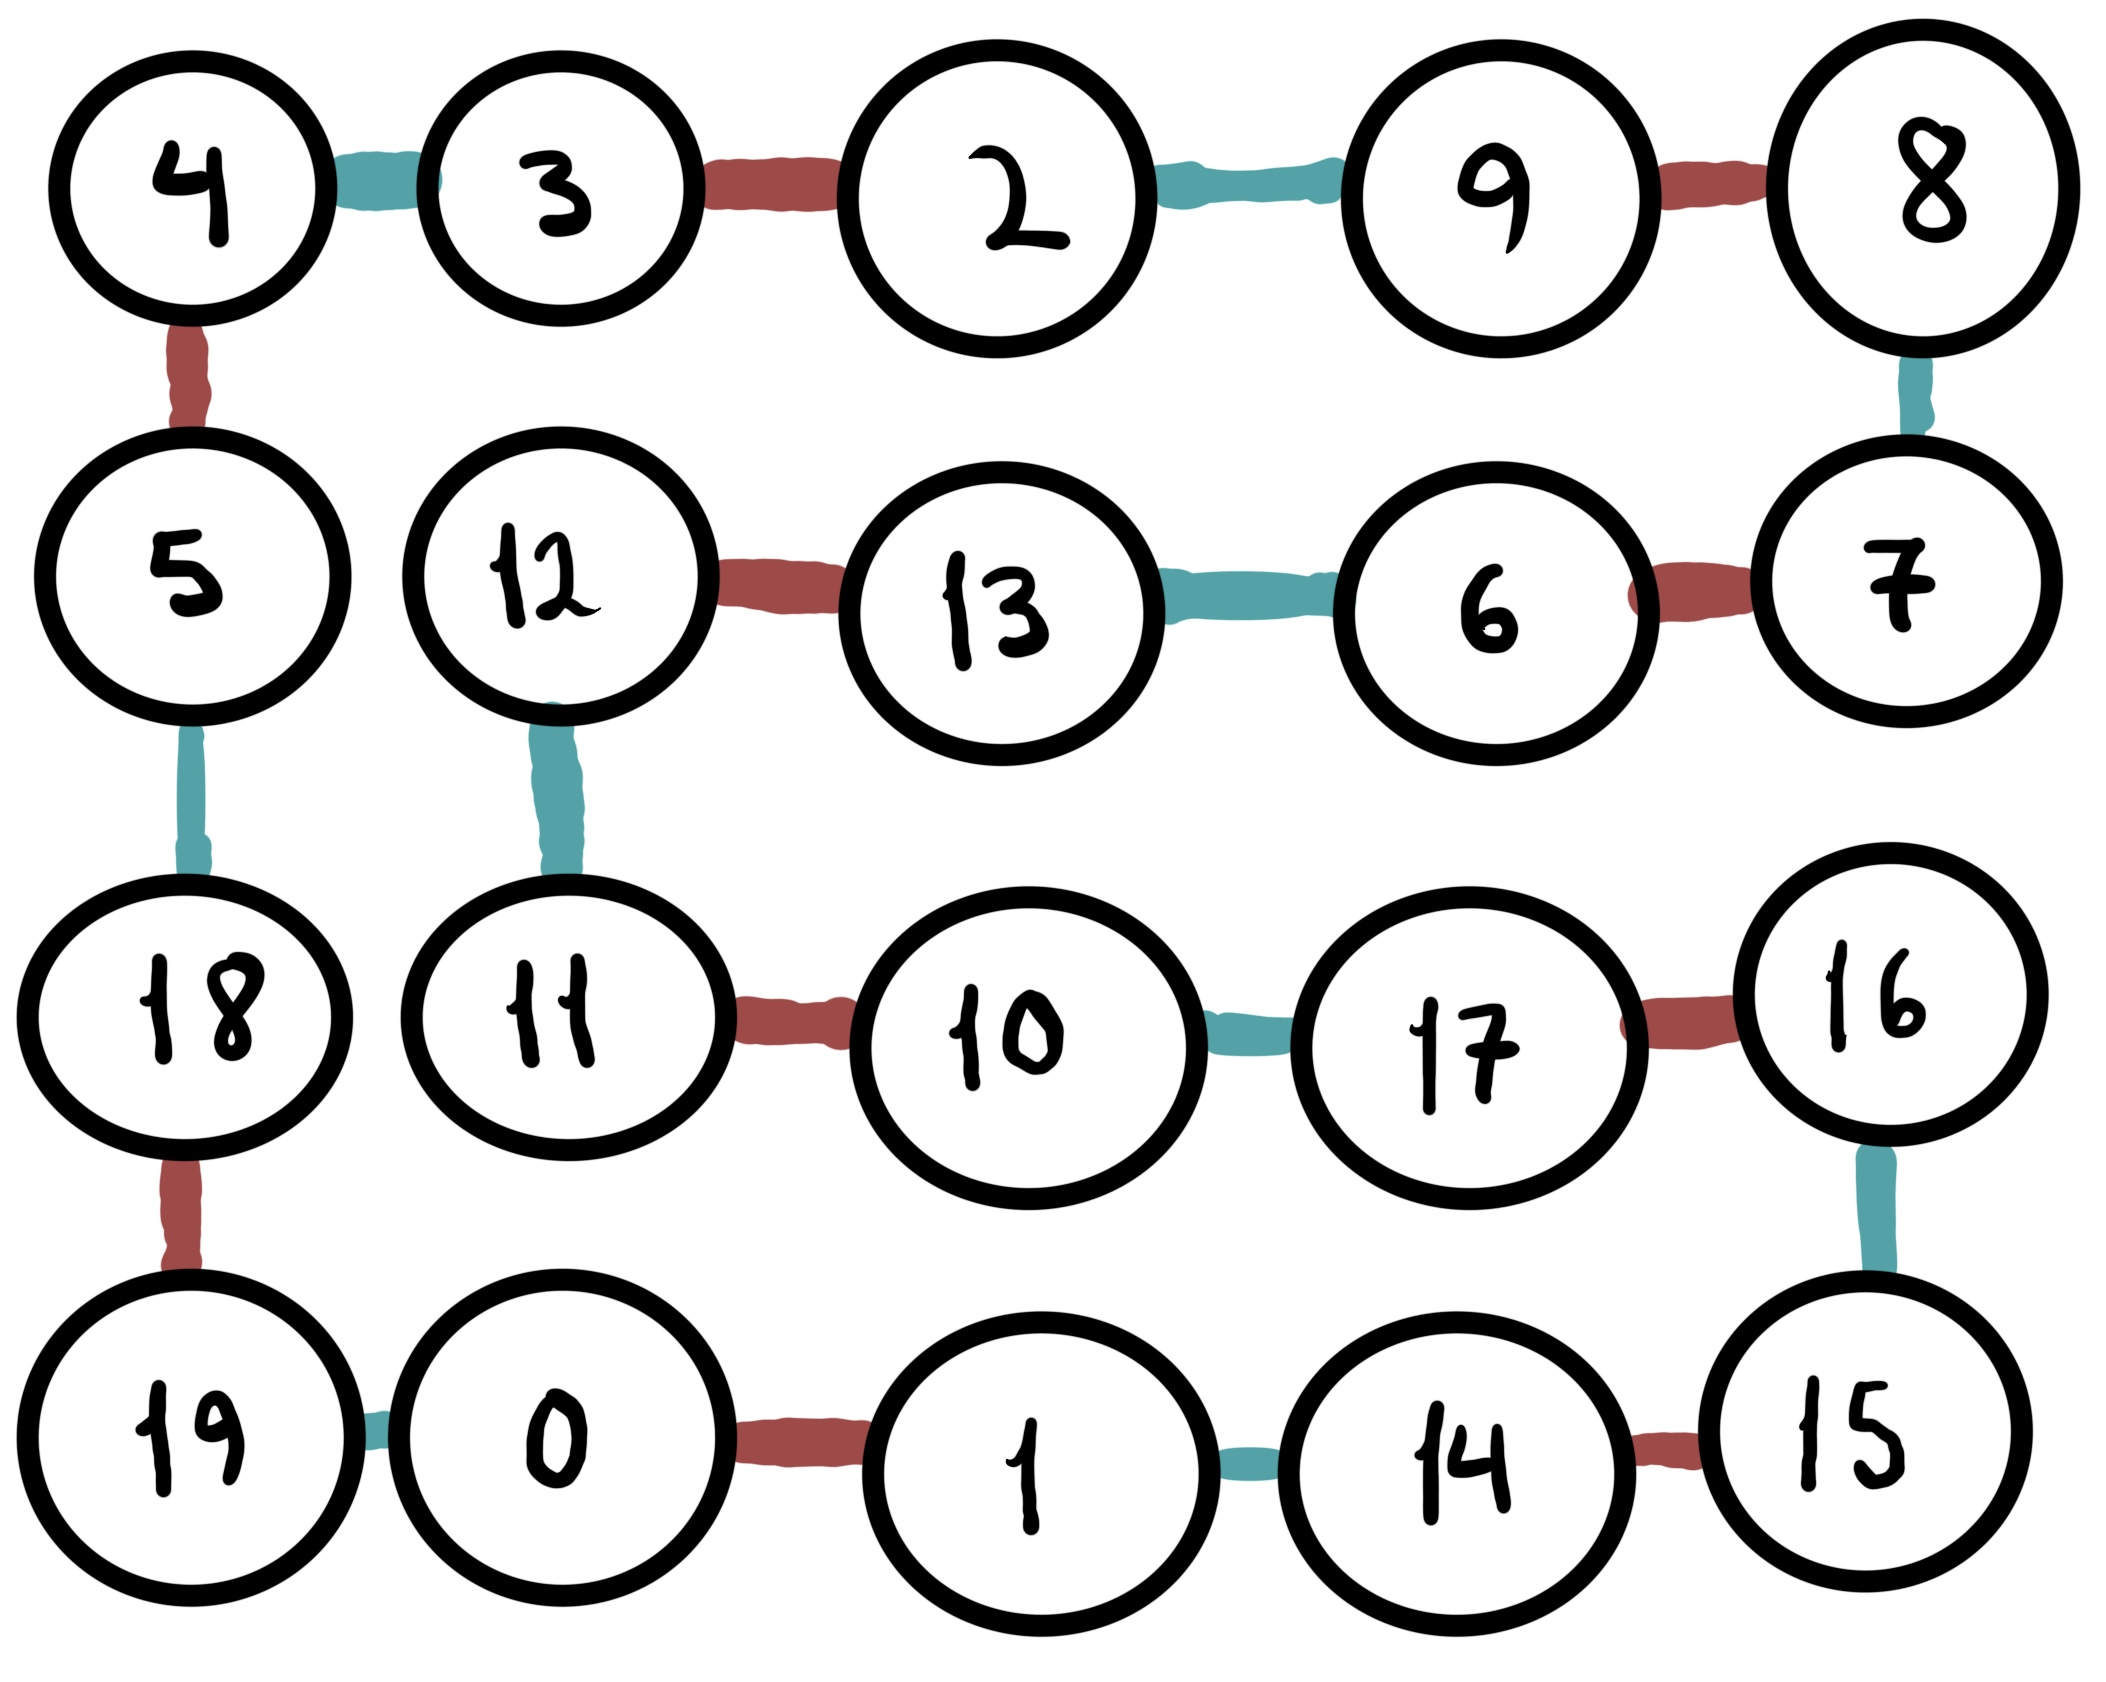
\includegraphics[scale=.05]{images/simplex-ring.jpg}
                \caption{Single topology}
                \end{subfigure}
                \begin{subfigure}[b]{.2\textwidth}
                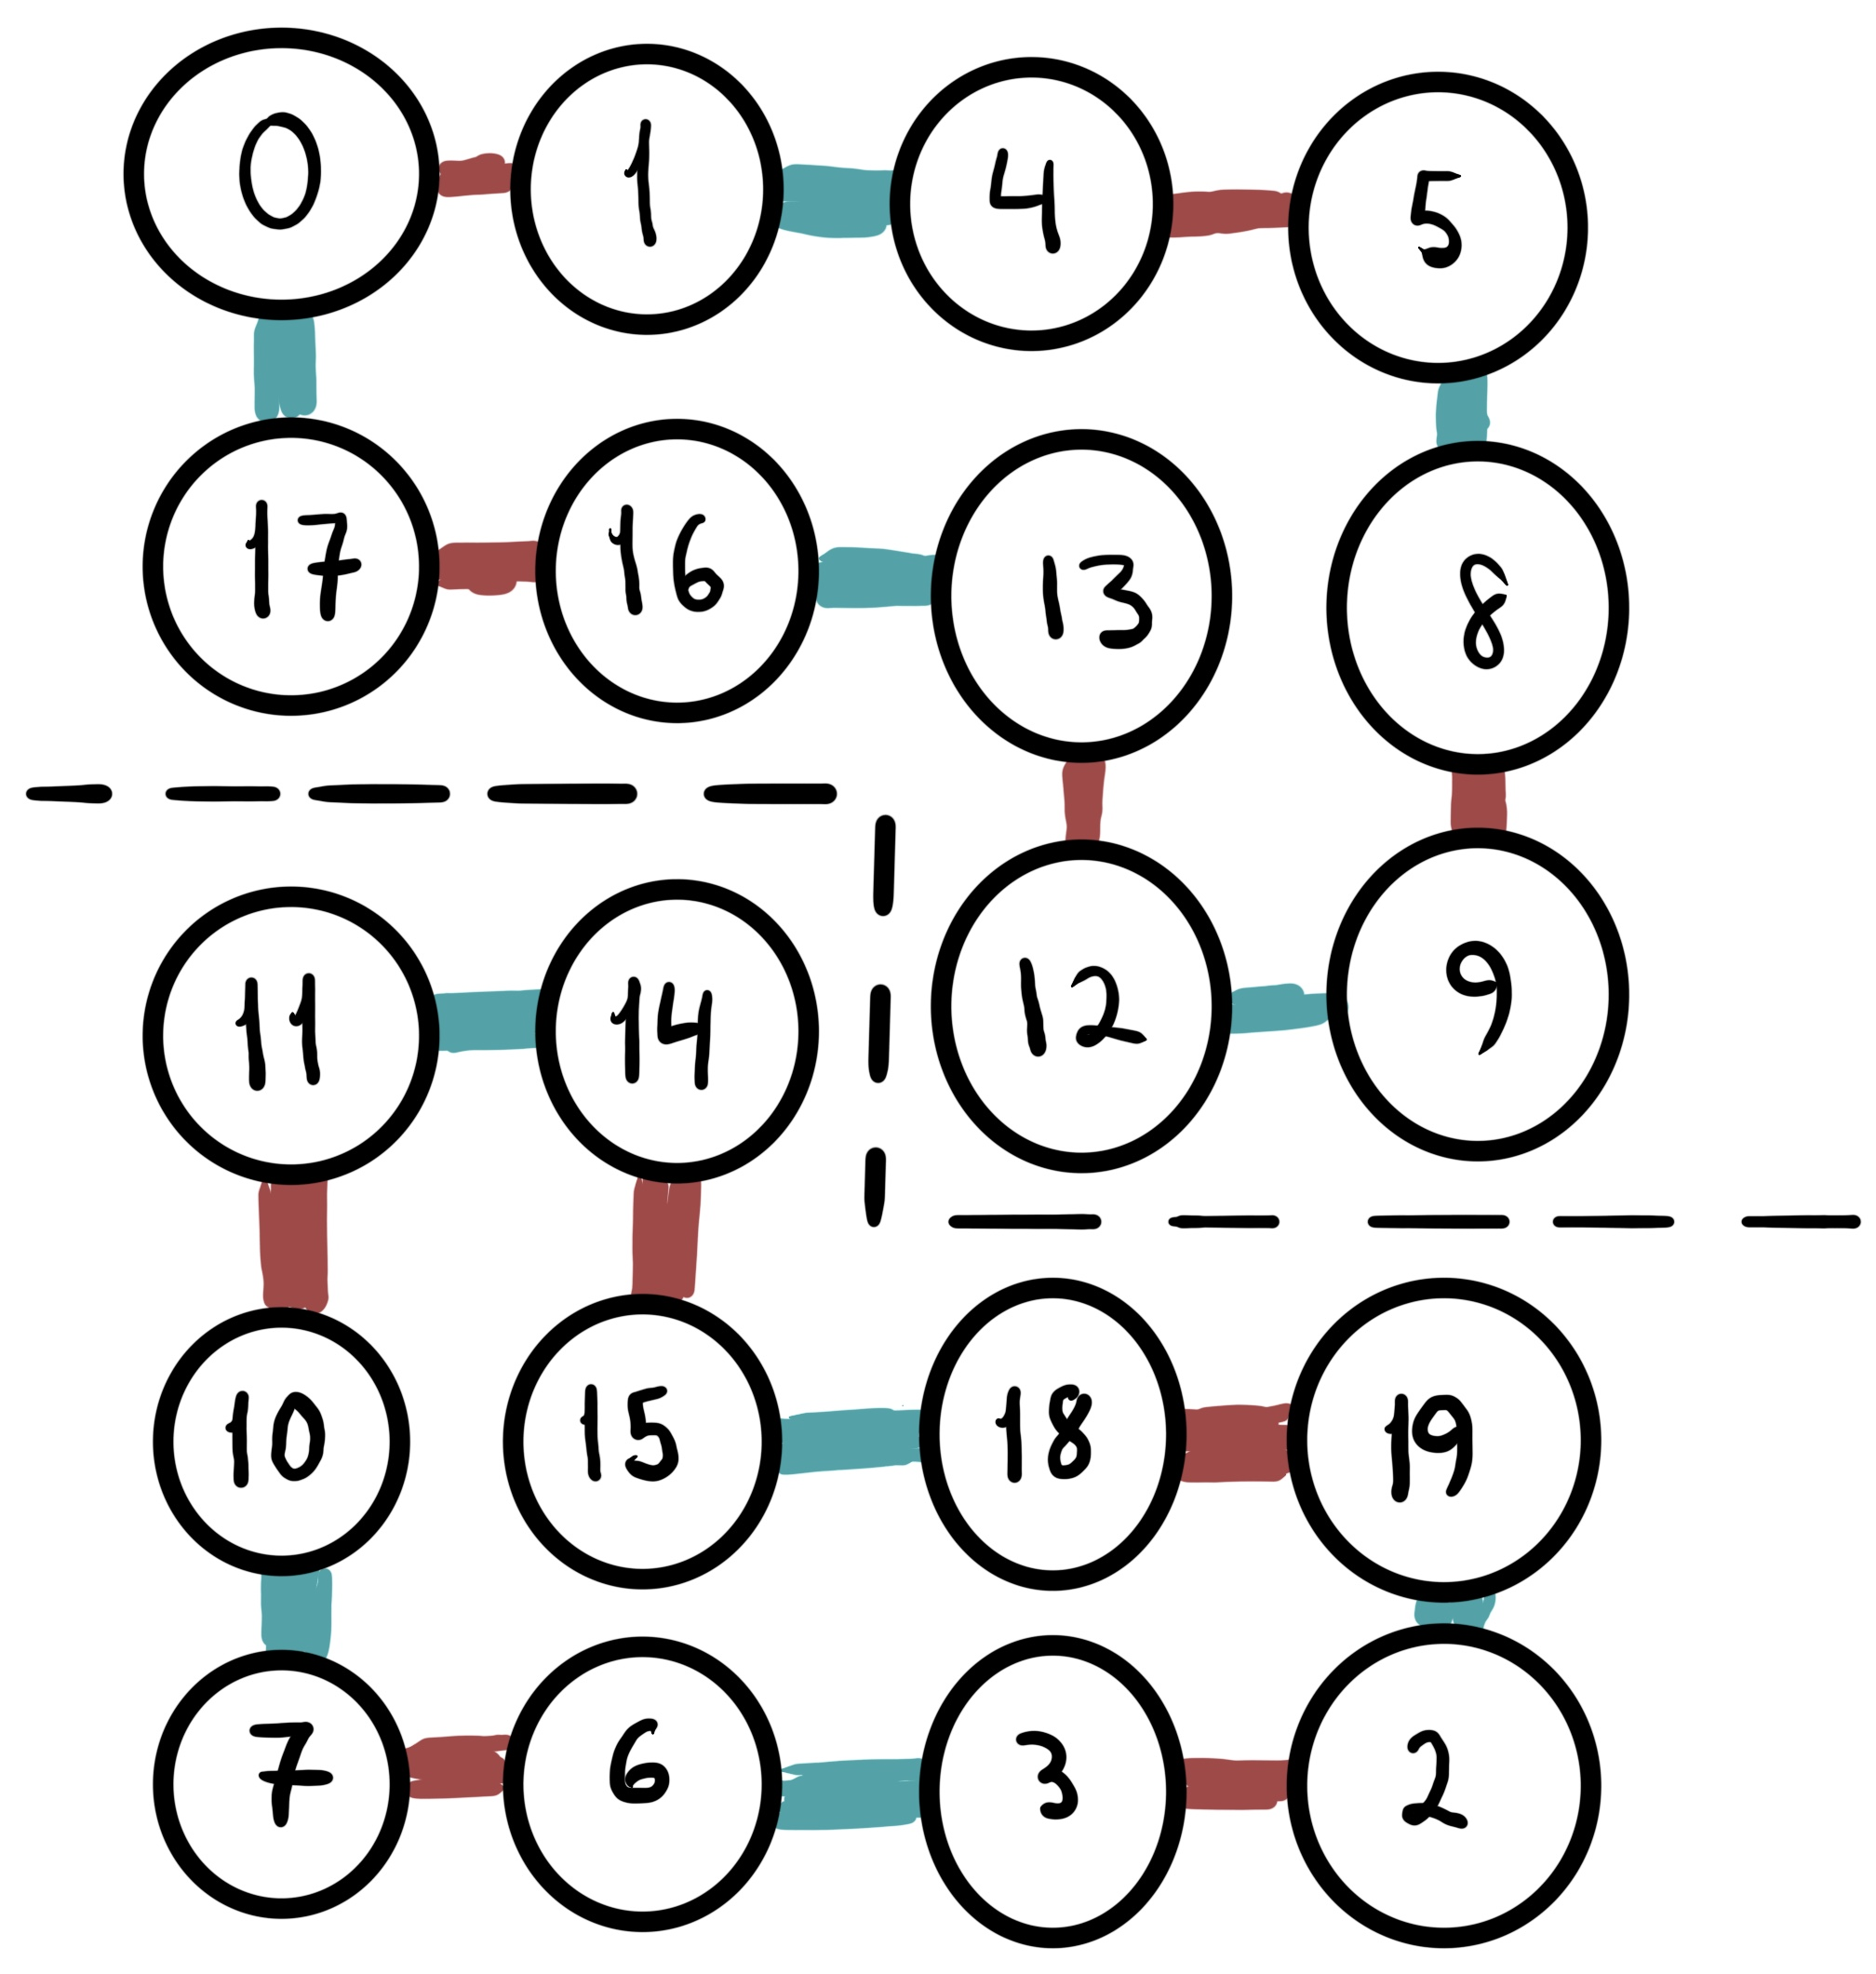
\includegraphics[scale=.05]{images/simplex-donuts.jpg}
                \caption{Double topology}
                \end{subfigure}
                \begin{subfigure}[b]{.3\textwidth}
                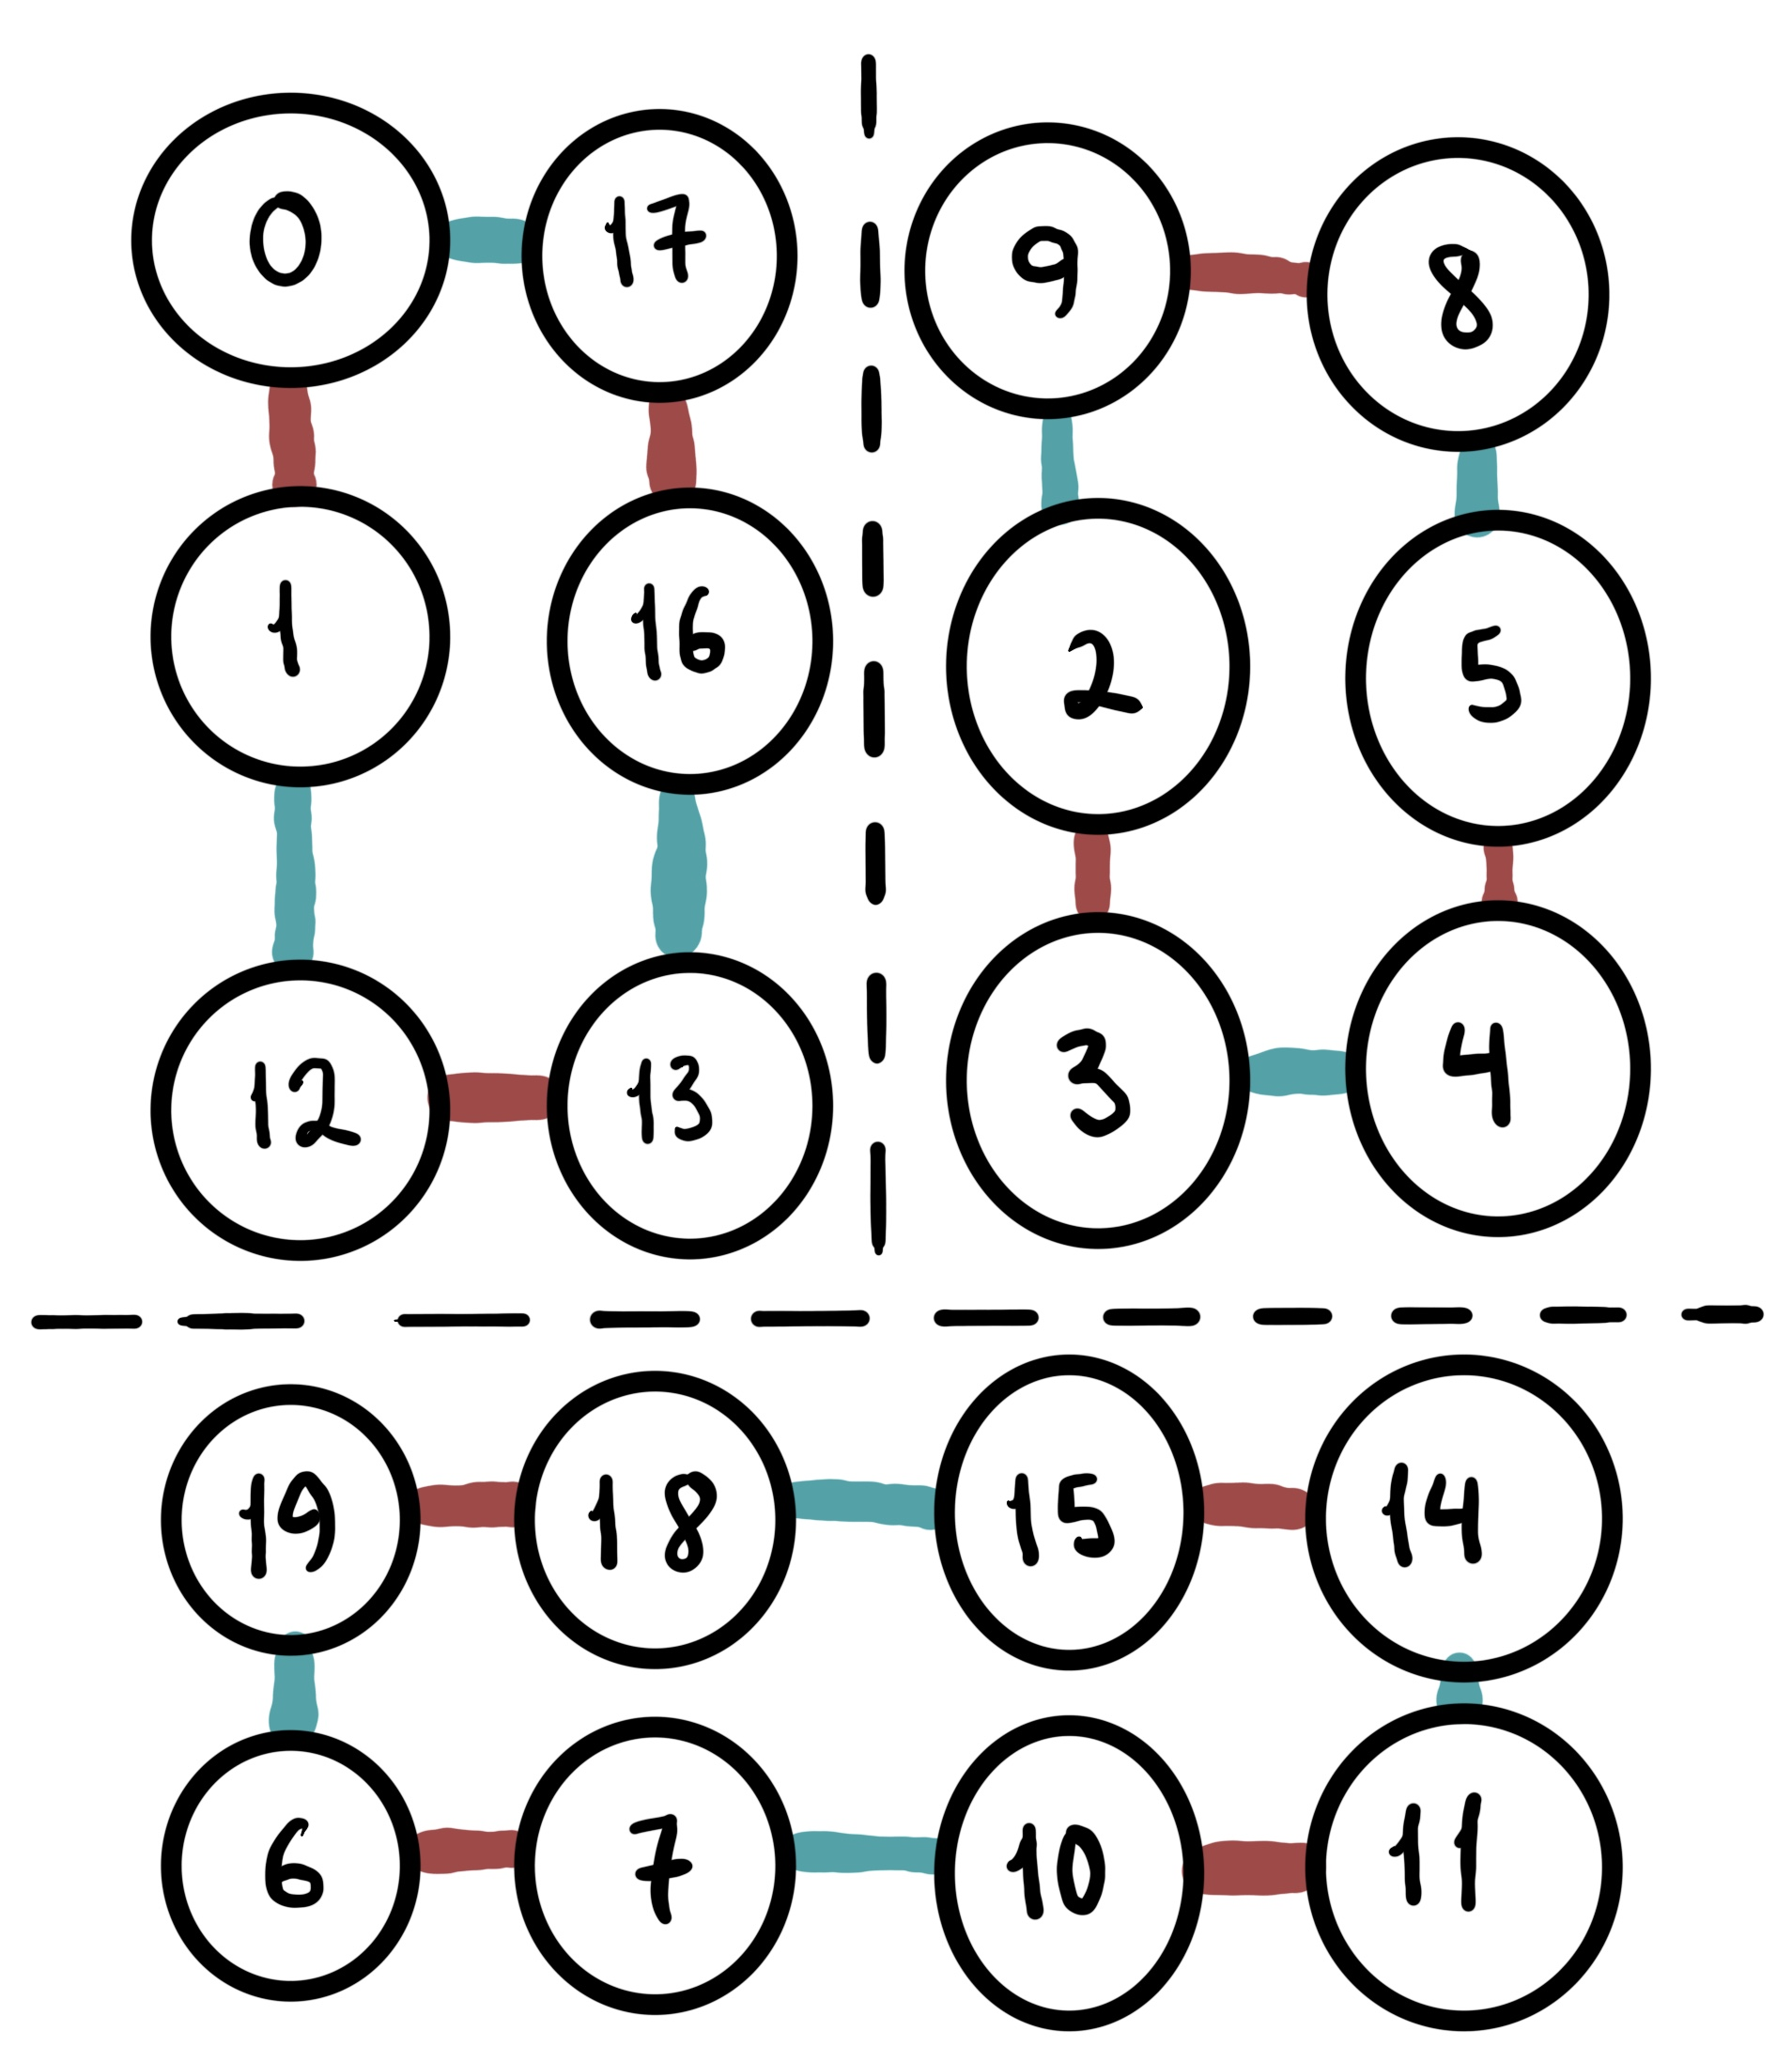
\includegraphics[scale=.05]{images/simplex-beans.jpg}
                \caption{Triple topology}
                \end{subfigure}
                \caption{4-simplex topology}
        \end{figure}        


\section{Results}
\subsection{State Preparation}
        
        \begin{table}[h]
        \begin{centering}
                \begin{tabular}{|l|l|}
                        \hline
                       $\bra{1_{L}}\ket{1_{L\text{sim}}} $ & $\bra{0_L}\ket{0_{L\text{sim}}}$\\ \hline
                       $0.8618$ & $0.9938$\\ \hline
                \end{tabular}
                \caption{State preparation fidelity}
        \end{centering}
        \end{table}
        The $\ket{1_L}$ and $\ket{0_L}$ state were each prepared 1000 times and their wavefunctions calculated. Above is the 
        dot product with the Hermetian conjugate with the numerically calculated expected wavefunction. This 
        fidelity is much higher than anything seen in the other literature \cite{ibm-qsim-qubit-of-space},\cite{qspacetime-on-qsim}.

\subsection{Submission One}        
        As of now, we have only received experiment results from one experiment with the QPU, to varying 
        degrees of success. 

        \subsubsection{QPU Qubit Malfunction}
        Unfortunately, there was an error on Weber's $(4,8)$ qubit. Every time this qubit was used as a control,
        it would reset the target qubit to zero. The target qubit would then encounter an $X$ flip in the inverse Bell 
        state phase, resulting in a 
        qubit with a final state of $1$ for every run. We used the qubit on every experiment except for the state preparation 
        and the single-chain dipole network, meaning those experiments are the only ones with useful results.

        \subsubsection{Single-Chain Dipole}
        Averaged over one-hundred thousand runs, the results of the single-chain dipole, figure 2.c, are shown below. 
        The expected amplitude is $0.015625$. The final state is always expected to have an even parity, so that can be used for post selection.
        \begin{table}[h]
        \begin{centering}
                \begin{tabular}{|l|l|l|}
                        \hline
                        & Results & Post-selected\\ \hline
                        $\abs{\bra{W}\ket{00_L}}^2$ & 0.01151 & 0.01869\\ \hline
                        Percent error &  26.336\%& 16.616\% \\\hline
                \end{tabular}
                \caption{$\bra{0\dots0}B^\dagger_{04,17,25,36}U\ket{0\dots 0}$}
        \end{centering}
        \end{table}

        Note that if the post-selected and non-post-selected results were averaged, we 
        would get $\abs{\bra{W}\ket{0_L0_L}}^2=0.01510$, which is percent error $=03.365\%$. 

        The $1$ state is much more unstable than the $0$ state, which means that many error channels,
         such as photon loss, will bias the $0$ state\cite{photon-loss}. Therefore, when we post-select 
        on the even parity, only errors where at least one  $1$ state is present are removed. However, many 
        of our errors are likely causing extra occurrences of the $\ket{0\dots0}$ state, which will not be removed.
        In order to combat this on the second submission, the $X$ gates at the end of the inverse Bell state were 
        changed such that we are looking for states of half zeros and half ones to count the amplitude of 
        $\ket{0\dots0}$. This way, the amplitude would not be overinflated by post-selection.

\subsection{Discussion and Future Work}
        Our simulations for the first submission were relatively simple, and closer to a trivial case. They  
        form a simple 3-dimensional boundary for 3+1 dimensional space-time, and the simulated spin-foam amplitudes are 
        a measure of the dynamics of quantum geometries in that space-time.

        Even though the first submission did not return many results, the work is promising. As can be seen in the single-chain 
        dipole network, results directly from the QPU are very close to the theoretically expected results. This 
        problem is especially promising to be successful on a quantum computer because it has a short runtime--
        the circuit has less than ten moments when converted to the $\sqrt{\text{iSWAP}}$ gate set. This gives the algorithm 
        high resistance to the low coherence times that frequently occur in superconductors, giving it promising prospects for NISQ computing.

        There is still a substantial amount of work to be further done. Next, we will create some formal proofs  
        the topological properties of the circuits. A state preparation circuit with better fidelity for $\ket{t(\theta\neq0)}$ 
        will be found, which will hopefully lead to high-fidelity simulations involving a qubit of space in 
        superposition of the $\ket{0_L}$ and $\ket{1_L}$ state. This would allow us to run the above algorithm with 
        spacetime tetrahedra which are eigenstates of the volume operator, $\ket{V_\pm} = \frac{\ket{0_L}\mp i\ket{1_L}}{\sqrt{2}}$ \cite{covariant-lqg}.
        We will also attempt to glue two space-time atoms together, as can be seen in \cite{two-vertex-sfa}, but with the larger 40 qubit system.


        

\vspace{0cm}
\bibliographystyle{ieeetr}
\begin{thebibliography}{99}
\bibitem{nisq}        
        J. Preskill,
        ``Quantum Computing in the NISQ era and beyond'',
        Quantum {\bf 2}, 79 (2018)
        [arXiv:1801.00862v3].

\bibitem{supremacy}
        F. Arute, K. Arya, et al.,
        ``Quantum supremacy using a programmable superconducting processor'',
        Nature {\bf 574}, 505-510 (2019).


\bibitem{ashketar}        
        A. Ashtekar and J. Lewandowski, Class. Quant. Grav. {\bf 21},
        R53 (2004) [gr-qc/0404018].

\bibitem{ibm-qsim-qubit-of-space}
        G. Czelusta, J. Mielczarek,
        ``Quantum simulations of a qubit of space'',
        Phys. Rev. {\bf D103}, 046001 (2021)
        [arXiv:2003.13124].

        %4

\bibitem{covariant-lqg}        
        C. Rovelli, F. Vidotto,
        ``Covariant Loop Quantum Gravity: An elementary introduction to Quantum Gravity and Spinfoam Theory'',
        Cambridge Monographs on Mathematical Physics, 2014.

\bibitem{diffeo}
        A. Ashtekar, J. Lewandowski, D. Marolf, J. Mourão, and T. Thiemann, 
        “Quantization of diffeomorphism invariant theories of connections with local degrees of freedom,” 
        Journal of mathematical physics,
         vol. 36, no. 11, pp. 6456–6493, 1995, doi: 10.1063/1.531252.

\bibitem{simplical-decomp}        
        S. Lawphongpanich, n.d., 
        Simplicial decompositionSimplicial Decomposition, 
        Encyclopedia of Optimization, Boston, MA, Springer US, pp. 2375-2378


        %8

\bibitem{qspacetime-on-qsim}        
        K. Li, Y. Li, M. Han, et al.,
        ``Quantum spacetime on a quantum simulator'',
        Communications Physics {\bf 2}, 122 (2019)


\bibitem{gluing-polyhedra}        
        B. Bayatas, E. Bianchi, N. Yokomizo,
        ``Gluing polyhedra with entanglement in loop quantum gravity'',
        Physical Review, {\bf D98}, 026001 (2018)

\bibitem{ooguri}        
        Ooguri, ``H. Topological lattice models in four-dimensions''. 
        Mod. Phys. Lett. {\bf A7}, 2799–2810 (1992).

\bibitem{adiabatic}
        J. Mielczarek,
        ``Spin networks on adiabatic quantum computer'',
        (2018) [arXiv:1801.06017].


\bibitem{homogeneity-lqc}        
        C. Rovelli, F. Vidotto,
        ``Stepping out of Homogeneity in Loop Quantum Cosmology'',
        Class.Quant.Grav.25:225014, (2008)
        [arXiv:0805.4585]



\bibitem{photon-loss}        
        I. Diniz, R. Sousa, 
        ``Intrinsic Photon Loss at the Interface of Superconducting Devices'',
        Phys. Rev. Lett. {\bf 125},  147702 (2020)

        
\bibitem{two-vertex-sfa}        
        P. Zhang, Z. Huang, C. Song, et al.,
        ``Observation of Two-vertex Four-Dimensional Spin Foam Amplitudes with a 10-qubit Superconducting Quantum Processor'',
        (2020)
        [arXiv:2007.13682]



%\bibitem{prelim-qsim-ibm}
%        J. Mielczarek,
%        ``Spin Foam Vertex Amplitudes on Quantum Computer -- Preliminary Results'',
%        (2019) [arXiv:1810.07100].  




\bibitem{cirq}        
        Cirq Developers. 
        Cirq (Version v0.10.0).
        Zenodo.
        (2021, March 5). http://doi.org/10.5281/zenodo.4586899






\end{thebibliography}  

\end{document} 